%% bare_jrnl.tex
%% V1.4
%% 2012/12/27
%% by Michael Shell
%% see http://www.michaelshell.org/
%% for current contact information.
%%
%% This is a skeleton file demonstrating the use of IEEEtran.cls
%% (requires IEEEtran.cls version 1.8 or later) with an IEEE journal paper.
%%
%% Support sites:
%% http://www.michaelshell.org/tex/ieeetran/
%% http://www.ctan.org/tex-archive/macros/latex/contrib/IEEEtran/
%% and
%% http://www.ieee.org/



% *** Authors should verify (and, if needed, correct) their LaTeX system  ***
% *** with the testflow diagnostic prior to trusting their LaTeX platform ***
% *** with production work. IEEE's font choices can trigger bugs that do  ***
% *** not appear when using other class files.                            ***
% The testflow support page is at:
% http://www.michaelshell.org/tex/testflow/


%%*************************************************************************
%% Legal Notice:
%% This code is offered as-is without any warranty either expressed or
%% implied; without even the implied warranty of MERCHANTABILITY or
%% FITNESS FOR A PARTICULAR PURPOSE!
%% User assumes all risk.
%% In no event shall IEEE or any contributor to this code be liable for
%% any damages or losses, including, but not limited to, incidental,
%% consequential, or any other damages, resulting from the use or misuse
%% of any information contained here.
%%
%% All comments are the opinions of their respective authors and are not
%% necessarily endorsed by the IEEE.
%%
%% This work is distributed under the LaTeX Project Public License (LPPL)
%% ( http://www.latex-project.org/ ) version 1.3, and may be freely used,
%% distributed and modified. A copy of the LPPL, version 1.3, is included
%% in the base LaTeX documentation of all distributions of LaTeX released
%% 2003/12/01 or later.
%% Retain all contribution notices and credits.
%% ** Modified files should be clearly indicated as such, including  **
%% ** renaming them and changing author support contact information. **
%%
%% File list of work: IEEEtran.cls, IEEEtran_HOWTO.pdf, bare_adv.tex,
%%                    bare_conf.tex, bare_jrnl.tex, bare_jrnl_compsoc.tex,
%%                    bare_jrnl_transmag.tex
%%*************************************************************************

% Note that the a4paper option is mainly intended so that authors in
% countries using A4 can easily print to A4 and see how their papers will
% look in print - the typesetting of the document will not typically be
% affected with changes in paper size (but the bottom and side margins will).
% Use the testflow package mentioned above to verify correct handling of
% both paper sizes by the user's LaTeX system.
%
% Also note that the "draftcls" or "draftclsnofoot", not "draft", option
% should be used if it is desired that the figures are to be displayed in
% draft mode.
%
\documentclass[journal]{IEEEtran}
%
% If IEEEtran.cls has not been installed into the LaTeX system files,
% manually specify the path to it like:
%\documentclass[journal]{../sty/IEEEtran}





% Some very useful LaTeX packages include:
% (uncomment the ones you want to load)


% *** MISC UTILITY PACKAGES ***
%
%\usepackage{ifpdf}
% Heiko Oberdiek's ifpdf.sty is very useful if you need conditional
% compilation based on whether the output is pdf or dvi.
% usage:
% \ifpdf
%   % pdf code
% \else
%   % dvi code
% \fi
% The latest version of ifpdf.sty can be obtained from:
% http://www.ctan.org/tex-archive/macros/latex/contrib/oberdiek/
% Also, note that IEEEtran.cls V1.7 and later provides a builtin
% \ifCLASSINFOpdf conditional that works the same way.
% When switching from latex to pdflatex and vice-versa, the compiler may
% have to be run twice to clear warning/error messages.






% *** CITATION PACKAGES ***
%
\usepackage{cite}
% cite.sty was written by Donald Arseneau
% V1.6 and later of IEEEtran pre-defines the format of the cite.sty package
% \cite{} output to follow that of IEEE. Loading the cite package will
% result in citation numbers being automatically sorted and properly
% "compressed/ranged". e.g., [1], [9], [2], [7], [5], [6] without using
% cite.sty will become [1], [2], [5]--[7], [9] using cite.sty. cite.sty's
% \cite will automatically add leading space, if needed. Use cite.sty's
% noadjust option (cite.sty V3.8 and later) if you want to turn this off
% such as if a citation ever needs to be enclosed in parenthesis.
% cite.sty is already installed on most LaTeX systems. Be sure and use
% version 4.0 (2003-05-27) and later if using hyperref.sty. cite.sty does
% not currently provide for hyperlinked citations.
% The latest version can be obtained at:
% http://www.ctan.org/tex-archive/macros/latex/contrib/cite/
% The documentation is contained in the cite.sty file itself.






% *** GRAPHICS RELATED PACKAGES ***
%
\ifCLASSINFOpdf
 \usepackage[pdftex]{graphicx}
  % declare the path(s) where your graphic files are
 \graphicspath{{../pdf/}{../jpeg/}}
  % and their extensions so you won't have to specify these with
  % every instance of \includegraphics
\DeclareGraphicsExtensions{.pdf,.jpeg,.png}
\else
  % or other class option (dvipsone, dvipdf, if not using dvips). graphicx
  % will default to the driver specified in the system graphics.cfg if no
  % driver is specified.
\usepackage[dvips]{graphicx}
  % declare the path(s) where your graphic files are
\graphicspath{{../eps/}}
  % and their extensions so you won't have to specify these with
  % every instance of \includegraphics
\DeclareGraphicsExtensions{.eps}
\fi
% graphicx was written by David Carlisle and Sebastian Rahtz. It is
% required if you want graphics, photos, etc. graphicx.sty is already
% installed on most LaTeX systems. The latest version and documentation
% can be obtained at:
% http://www.ctan.org/tex-archive/macros/latex/required/graphics/
% Another good source of documentation is "Using Imported Graphics in
% LaTeX2e" by Keith Reckdahl which can be found at:
% http://www.ctan.org/tex-archive/info/epslatex/
%
% latex, and pdflatex in dvi mode, support graphics in encapsulated
% postscript (.eps) format. pdflatex in pdf mode supports graphics
% in .pdf, .jpeg, .png and .mps (metapost) formats. Users should ensure
% that all non-photo figures use a vector format (.eps, .pdf, .mps) and
% not a bitmapped formats (.jpeg, .png). IEEE frowns on bitmapped formats
% which can result in "jaggedy"/blurry rendering of lines and letters as
% well as large increases in file sizes.
%
% You can find documentation about the pdfTeX application at:
% http://www.tug.org/applications/pdftex





% *** MATH PACKAGES ***
%
\usepackage[cmex10]{amsmath}
% A popular package from the American Mathematical Society that provides
% many useful and powerful commands for dealing with mathematics. If using
% it, be sure to load this package with the cmex10 option to ensure that
% only type 1 fonts will utilized at all point sizes. Without this option,
% it is possible that some math symbols, particularly those within
% footnotes, will be rendered in bitmap form which will result in a
% document that can not be IEEE Xplore compliant!
%
% Also, note that the amsmath package sets \interdisplaylinepenalty to 10000
% thus preventing page breaks from occurring within multiline equations. Use:
%\interdisplaylinepenalty=2500
% after loading amsmath to restore such page breaks as IEEEtran.cls normally
% does. amsmath.sty is already installed on most LaTeX systems. The latest
% version and documentation can be obtained at:
% http://www.ctan.org/tex-archive/macros/latex/required/amslatex/math/





% *** SPECIALIZED LIST PACKAGES ***
%
\usepackage{algorithmic}
% algorithmic.sty was written by Peter Williams and Rogerio Brito.
% This package provides an algorithmic environment fo describing algorithms.
% You can use the algorithmic environment in-text or within a figure
% environment to provide for a floating algorithm. Do NOT use the algorithm
% floating environment provided by algorithm.sty (by the same authors) or
% algorithm2e.sty (by Christophe Fiorio) as IEEE does not use dedicated
% algorithm float types and packages that provide these will not provide
% correct IEEE style captions. The latest version and documentation of
% algorithmic.sty can be obtained at:
% http://www.ctan.org/tex-archive/macros/latex/contrib/algorithms/
% There is also a support site at:
% http://algorithms.berlios.de/index.html
% Also of interest may be the (relatively newer and more customizable)
% algorithmicx.sty package by Szasz Janos:
% http://www.ctan.org/tex-archive/macros/latex/contrib/algorithmicx/




% *** ALIGNMENT PACKAGES ***
%
\usepackage{array}
% Frank Mittelbach's and David Carlisle's array.sty patches and improves
% the standard LaTeX2e array and tabular environments to provide better
% appearance and additional user controls. As the default LaTeX2e table
% generation code is lacking to the point of almost being broken with
% respect to the quality of the end results, all users are strongly
% advised to use an enhanced (at the very least that provided by array.sty)
% set of table tools. array.sty is already installed on most systems. The
% latest version and documentation can be obtained at:
% http://www.ctan.org/tex-archive/macros/latex/required/tools/


% IEEEtran contains the IEEEeqnarray family of commands that can be used to
% generate multiline equations as well as matrices, tables, etc., of high
% quality.




% *** SUBFIGURE PACKAGES ***
\ifCLASSOPTIONcompsoc
  \usepackage[caption=false,font=normalsize,labelfont=sf,textfont=sf]{subfig}
\else
  \usepackage[caption=false,font=footnotesize]{subfig}
\fi
% subfig.sty, written by Steven Douglas Cochran, is the modern replacement
% for subfigure.sty, the latter of which is no longer maintained and is
% incompatible with some LaTeX packages including fixltx2e. However,
% subfig.sty requires and automatically loads Axel Sommerfeldt's caption.sty
% which will override IEEEtran.cls' handling of captions and this will result
% in non-IEEE style figure/table captions. To prevent this problem, be sure
% and invoke subfig.sty's "caption=false" package option (available since
% subfig.sty version 1.3, 2005/06/28) as this is will preserve IEEEtran.cls
% handling of captions.
% Note that the Computer Society format requires a larger sans serif font
% than the serif footnote size font used in traditional IEEE formatting
% and thus the need to invoke different subfig.sty package options depending
% on whether compsoc mode has been enabled.
%
% The latest version and documentation of subfig.sty can be obtained at:
% http://www.ctan.org/tex-archive/macros/latex/contrib/subfig/




% *** FLOAT PACKAGES ***
%
%\usepackage{fixltx2e}
% fixltx2e, the successor to the earlier fix2col.sty, was written by
% Frank Mittelbach and David Carlisle. This package corrects a few problems
% in the LaTeX2e kernel, the most notable of which is that in current
% LaTeX2e releases, the ordering of single and double column floats is not
% guaranteed to be preserved. Thus, an unpatched LaTeX2e can allow a
% single column figure to be placed prior to an earlier double column
% figure. The latest version and documentation can be found at:
% http://www.ctan.org/tex-archive/macros/latex/base/


%\usepackage{stfloats}
% stfloats.sty was written by Sigitas Tolusis. This package gives LaTeX2e
% the ability to do double column floats at the bottom of the page as well
% as the top. (e.g., "\begin{figure*}[!b]" is not normally possible in
% LaTeX2e). It also provides a command:
%\fnbelowfloat
% to enable the placement of footnotes below bottom floats (the standard
% LaTeX2e kernel puts them above bottom floats). This is an invasive package
% which rewrites many portions of the LaTeX2e float routines. It may not work
% with other packages that modify the LaTeX2e float routines. The latest
% version and documentation can be obtained at:
% http://www.ctan.org/tex-archive/macros/latex/contrib/sttools/
% Do not use the stfloats baselinefloat ability as IEEE does not allow
% \baselineskip to stretch. Authors submitting work to the IEEE should note
% that IEEE rarely uses double column equations and that authors should try
% to avoid such use. Do not be tempted to use the cuted.sty or midfloat.sty
% packages (also by Sigitas Tolusis) as IEEE does not format its papers in
% such ways.
% Do not attempt to use stfloats with fixltx2e as they are incompatible.
% Instead, use Morten Hogholm'a dblfloatfix which combines the features
% of both fixltx2e and stfloats:
%
% \usepackage{dblfloatfix}
% The latest version can be found at:
% http://www.ctan.org/tex-archive/macros/latex/contrib/dblfloatfix/




%\ifCLASSOPTIONcaptionsoff
%  \usepackage[nomarkers]{endfloat}
% \let\MYoriglatexcaption\caption
% \renewcommand{\caption}[2][\relax]{\MYoriglatexcaption[#2]{#2}}
%\fi
% endfloat.sty was written by James Darrell McCauley, Jeff Goldberg and
% Axel Sommerfeldt. This package may be useful when used in conjunction with
% IEEEtran.cls'  captionsoff option. Some IEEE journals/societies require that
% submissions have lists of figures/tables at the end of the paper and that
% figures/tables without any captions are placed on a page by themselves at
% the end of the document. If needed, the draftcls IEEEtran class option or
% \CLASSINPUTbaselinestretch interface can be used to increase the line
% spacing as well. Be sure and use the nomarkers option of endfloat to
% prevent endfloat from "marking" where the figures would have been placed
% in the text. The two hack lines of code above are a slight modification of
% that suggested by in the endfloat docs (section 8.4.1) to ensure that
% the full captions always appear in the list of figures/tables - even if
% the user used the short optional argument of \caption[]{}.
% IEEE papers do not typically make use of \caption[]'s optional argument,
% so this should not be an issue. A similar trick can be used to disable
% captions of packages such as subfig.sty that lack options to turn off
% the subcaptions:
% For subfig.sty:
% \let\MYorigsubfloat\subfloat
% \renewcommand{\subfloat}[2][\relax]{\MYorigsubfloat[]{#2}}
% However, the above trick will not work if both optional arguments of
% the \subfloat command are used. Furthermore, there needs to be a
% description of each subfigure *somewhere* and endfloat does not add
% subfigure captions to its list of figures. Thus, the best approach is to
% avoid the use of subfigure captions (many IEEE journals avoid them anyway)
% and instead reference/explain all the subfigures within the main caption.
% The latest version of endfloat.sty and its documentation can obtained at:
% http://www.ctan.org/tex-archive/macros/latex/contrib/endfloat/
%
% The IEEEtran \ifCLASSOPTIONcaptionsoff conditional can also be used
% later in the document, say, to conditionally put the References on a
% page by themselves.




% *** PDF, URL AND HYPERLINK PACKAGES ***
%
%\usepackage{url}
% url.sty was written by Donald Arseneau. It provides better support for
% handling and breaking URLs. url.sty is already installed on most LaTeX
% systems. The latest version and documentation can be obtained at:
% http://www.ctan.org/tex-archive/macros/latex/contrib/url/
% Basically, \url{my_url_here}.




% *** Do not adjust lengths that control margins, column widths, etc. ***
% *** Do not use packages that alter fonts (such as pslatex).         ***
% There should be no need to do such things with IEEEtran.cls V1.6 and later.
% (Unless specifically asked to do so by the journal or conference you plan
% to submit to, of course. )


% correct bad hyphenation here
\hyphenation{op-tical net-works semi-conduc-tor}


\begin{document}
%
% paper title
% can use linebreaks \\ within to get better formatting as desired
% Do not put math or special symbols in the title.
\title{A Customized Real-time Compilation for Motion Control in Embedded PLCs}
%
%
% author names and IEEE memberships
% note positions of commas and nonbreaking spaces ( ~ ) LaTeX will not break
% a structure at a ~ so this keeps an author's name from being broken across
% two lines.
% use \thanks{} to gain access to the first footnote area
% a separate \thanks must be used for each paragraph as LaTeX2e's \thanks
% was not built to handle multiple paragraphs
%

\author{Huifeng Wu,
        Yi Yan, Danfeng Sun, Rene Simon% <-this % stops a space
\thanks{Huifeng Wu and Yi Yan are with the Institute of Intelligent and Software Technology, Hangzhou Dianzi University, Hangzhou, 310018, China (e-mail: yybjyyj@163.com).}% <-this % stops a space
\thanks{Danfeng Sun are with the Institute of Industrial Internet, Hangzhou Dianzi University, Hangzhou, 310018, China.}
\thanks{Rene Simon is with the Department of Automation and Computer Sciences, Harz University of Applied Sciences, Wernigerode, 38855, Germany.}
\thanks{This work was supported by a Grant from The National Natural Science Foundation of China(No.U1609211), Science and Technology Program of Zhejiang Province(No.2018C04001)}
}% <-this % stops a space
%\thanks{Manuscript received April 19, 2005; revised December 27, 2012.}}

% note the % following the last \IEEEmembership and also \thanks -
% these prevent an unwanted space from occurring between the last author name
% and the end of the author line. i.e., if you had this:
%
% \author{....lastname \thanks{...} \thanks{...} }
%                     ^------------^------------^----Do not want these spaces!
%
% a space would be appended to the last name and could cause every name on that
% line to be shifted left slightly. This is one of those "LaTeX things". For
% instance, "\textbf{A} \textbf{B}" will typeset as "A B" not "AB". To get
% "AB" then you have to do: "\textbf{A}\textbf{B}"
% \thanks is no different in this regard, so shield the last } of each \thanks
% that ends a line with a % and do not let a space in before the next \thanks.
% Spaces after \IEEEmembership other than the last one are OK (and needed) as
% you are supposed to have spaces between the names. For what it is worth,
% this is a minor point as most people would not even notice if the said evil
% space somehow managed to creep in.



% The paper headers

%\markboth{Journal of \LaTeX\ Class Files,~Vol.~11, No.~4, December~2012}%
%{Shell \MakeLowercase{\textit{et al.}}: Bare Demo of IEEEtran.cls for Journals}

% The only time the second header will appear is for the odd numbered pages
% after the title page when using the twoside option.
%
% *** Note that you probably will NOT want to include the author's ***
% *** name in the headers of peer review papers.                   ***
% You can use \ifCLASSOPTIONpeerreview for conditional compilation here if
% you desire.




% If you want to put a publisher's ID mark on the page you can do it like
% this:
%\IEEEpubid{0000--0000/00\$00.00~\copyright~2012 IEEE}
% Remember, if you use this you must call \IEEEpubidadjcol in the second
% column for its text to clear the IEEEpubid mark.



% use for special paper notices
%\IEEEspecialpapernotice{(Invited Paper)}




% make the title area
\maketitle

% As a general rule, do not put math, special symbols or citations
% in the abstract or keywords.
% * <karyns@accdon.com> 2017-12-24T08:35:37.488Z:
% 
% General note: Language was unclear in many areas. I have done my best to guess at your intended meaning. Please carefully review all edits. 
% 
% ^.
\begin{abstract}
General PLCs are difficult to adapt to changeable applications, especially for those with special motion control; this has seriously affected the development efficiency. This paper presents the concept of the embedded PLC (ePLC), whose hardware structure can be customized according to actual requirements. We proposed a three-layer architecture, and its customizable application layer could be compiled in real time. Correspondingly, the PLC program was divided into an engine program, control program, and customizing program. The description and compilation method of the customizing program was provided. We presented a customized winding machine language (CWML) based on the proposed ePLC software structure. This was implemented in an automatic winding machine, which was easier to use compared with some widely used languages (e.g., G-Code). 
% * <karyns@accdon.com> 2017-12-24T08:32:14.912Z:
% 
% > customizable application layer
% Original wording was weird. Please confirm  change.
% 
% ^.
% * <karyns@accdon.com> 2017-12-24T08:28:06.592Z:
% 
% > changeable applications
% Meaning is unclear. Do you mean  "applications with multiple functions" or "different applications"? Please reword/clarify. 
% 
% ^.
% * <karyns@accdon.com> 2017-12-24T08:27:24.430Z:
% 
% > PLCs
% Please define.
% 
% ^.
\end{abstract}

% Note that keywords are not normally used for peerreview papers.
\begin{IEEEkeywords}
motion control, customizing program, embedded PLC
\end{IEEEkeywords}

% For peer review papers, you can put extra information on the cover
% page as needed:
% \ifCLASSOPTIONpeerreview
% \begin{center} \bfseries EDICS Category: 3-BBND \end{center}
% \fi
%
% For peerreview papers, this IEEEtran command inserts a page break and
% creates the second title. It will be ignored for other modes.
\IEEEpeerreviewmaketitle



\section{Introduction}


PLCs are used for logic control in many applications\cite{A0,A1}. In order to meet the increasingly complex control needs, many scholars initiated research to improve PLC performance, such as enhancement through algorithms and corresponding function modules\cite{A2}, improving the safety and reliability of PLCs by improving certain design methods\cite{A3,A5,A34,A4}, and improving program quality through forecasting and finding mistakes in the control procedure \cite{A6}. Software development and verification methods for PLCs are important research subjects\cite{A42,A45,A46,A43,A44,A41}. In addition to improving the performance of PLCs, their functionality has also been enhanced with the fast development of integrated circuit technology. Now, PLCs have motion control abilities, such as position controlling, linear interpolation, and circular interpolation, for a wide range of applications\cite{A22,A18,A29,A28}. By integrating motion control into the PLC, the control system was greatly simplified because simple motion control can be realized by the PLC without a special motion controller. There are many ways to realize this integration. One is to integrate a simple motion control function into the PLC\cite{A20,A21}, which combines logic control and motion control. However, this hardly ensures the accuracy and speed of sophisticated motion control functions because the motion control and the logic control operate in the same cycle. Therefore, this approach is usually used in simple motion control applications. Another way to realize integration is to use an independent motion control module. The module has an independent executive system and development environment, and it can accomplish complex motion control by means of communication and interaction with the PLCs. An example of this is seen in the Panasonic FP2 position control unit\cite{A24}.


There are different ways to develop a PLC program with motion control. For motion control integrated into a PLC, the motion control program is developed in the PLC's development environment. For independent expansion motion modules, the motion control program can be developed by G-Code, such as in the MC421/221 of OMRON CS1 series PLC \cite{OMRON2006}. It can also be developed by special programming languages, such as the textual description language SYMPAS or provided by motion control instructions in ladder-diagram programming environments, such as the FP series PLC created by Panasonic \cite{A24}. In order to meet different applications needs, different controllers must be chosen, and specific development environments and development languages to accomplish the system design and development are required. This is a great challenge for designers. The motion control standard \cite{A12} provides a standard library that can be reused among different platforms, and can reduce the complexity and the costs of development and maintenance. Many present design tools adopt this development method, such as CoDeSys and MULTIPROG. CoDeSys SoftMotion combines PLC logical control with motion control \cite{3S2017}. It integrates a motion control function toolkit into the PLC programming system, and utilizes the IEC61131-3 standard programming language for development. It can also expand the CNC POU library to provide complex motion control functions such as interpolation.

Although the function of PLCs has been enhanced, especially in the field of complex motion control, there are still some shortcomings of PLCs. These are listed below.
\begin{enumerate}
	\item Since PLCs are designed for general purposes, they are not the optimal choice for a control task. Additionally, the development process of motion control in PLCs is not convenient, and the PLC requires continual reprogramming to meet the requirement of a specific application. Furthermore, although the IEC61131-3 standard development languages are suitable for developing a logic control program, it is challenging to develop complex motion control programs.
	\item Function development and process development are mixed together, which makes it hard to adjust the sequence and parameters. Function development refers to the development of some basic function, such as servo motor control, and the function is not related to any application. Meanwhile, process development refers to application-related development, such as the cooperation of servo motors. Function development always results in libraries. Under the traditional development architecture, developers should not only accomplish function development, but also need to be familiar with the process and technical parameters in the development of certain equipment control procedures, which greatly extends the development period.
	\item End-users cannot adjust the program according to actual control needs. End-users are most familiar with the actual requirement, and they always need to adjust the sequence and parameters of motion control to achieve optimal control. However, the existing development method does not support users to customize the program.
\end{enumerate}

In order to solve these problems and expand the scope of PLC applications, this paper puts forward the concept of an embedded PLC whose hardware structure can be customized according to actual requirements and whose software structure is divided into three layers, with an application layer that can be compiled in real time. The remainder of this paper is organized as follows. In section \ref{The-Basic-Ideology}, we introduce the basic ideology and concept of this paper. In sections \ref{Engine-Algorithms1}, \ref{ACP-PLC2} , \ref{PLC-Control-Program3}, and \ref{Collaboration-Threads}, we describe the implementation process in detail. A case analysis is carried out in section \ref{Case-Analysis}. Finally, conclusions and future work is discussed in section \ref{conclusion}.



\section{The Basic Ideology and Concept}
\label{The-Basic-Ideology}


\subsection{The Concept of ePLC}
With function enhancement of the embedded processor, it is possible to implement several control tasks in one or more embedded processors. The $ePLC$ takes the embedded processor as the core, and peripheral circuits can be added according to requirements. The $ePLC$ has more open hardware structure compared with PLCs, and its hardware can be customized on-demand, making it quite similar to a special controller. The software structure of $ePLC$ can also be customized. The development method of the $ePLC$ is similar to that of the PLC, which means that the languages of IEC61131-3 are also supported\cite{A40}. Fig. \ref{fig:multi_cpuPLC1} shows one typical structure of the $ePLC$. It contains three cores. The $ePLC$ has been applied in some fields (e.g., CAD \cite{Huifeng2015A}).

\begin{figure}
	\centering
	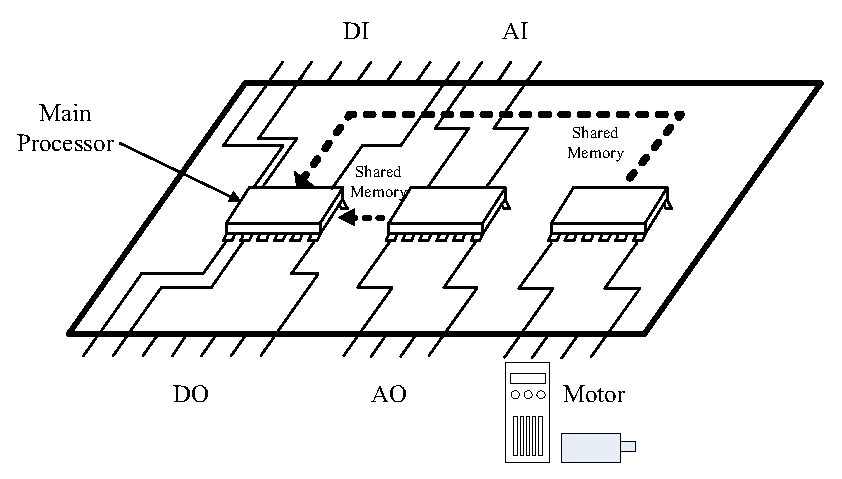
\includegraphics[width=3in]{fig/FIG1_TII-18-0024.eps}
	\caption{ Hardware structure of the $ePLC$.}
	\label{fig:multi_cpuPLC1}
\end{figure}
\subsection{Multilayer Architecture of ePLC}
 Fig. \ref{fig:controlblocks} shows that the general control program of PLCs includes several program blocks, and the execution flow is determined at design time. In our architecture, the control program also includes several program blocks, but they are independent from each other, which means that the execution flow is not determined at design time, and even the parameters can be adjusted, as  shown in Fig. \ref{fig:customeprogram}.

The execution flow can be changed without reprogramming the control program at runtime. To achieve this goal, a customizing program is introduced to the $ePLC$, and a customizing thread is added to the executing system of the $ePLC$ to parse and run the customizing program. The traditional PLC's executing system includes a control program driver module. This module interprets the input signals, carries out the program stored in memory, and generates the output signals; this process is an endless loop when the PLC is running. At the same time, communication, exception handling, and other functions are implemented in the loop. With the enhancement of PLC functionality and application complexity, the control program became more complicated. In order to improve the control efficiency, the PLC's executing system uses multiple threads progressively. A customizing thread can be added to the executing system to parse and run the customizing program in the multi-threads kernel.

\begin{figure}
\centering
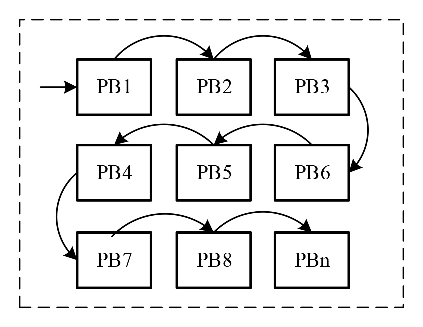
\includegraphics[width=2in]{fig/FIG2_TII-18-0024.eps}
\caption{ General control program of the PLC includes several program blocks, and the execution flow is determined at design time.}
\label{fig:controlblocks}
\end{figure}

\begin{figure}
\centering
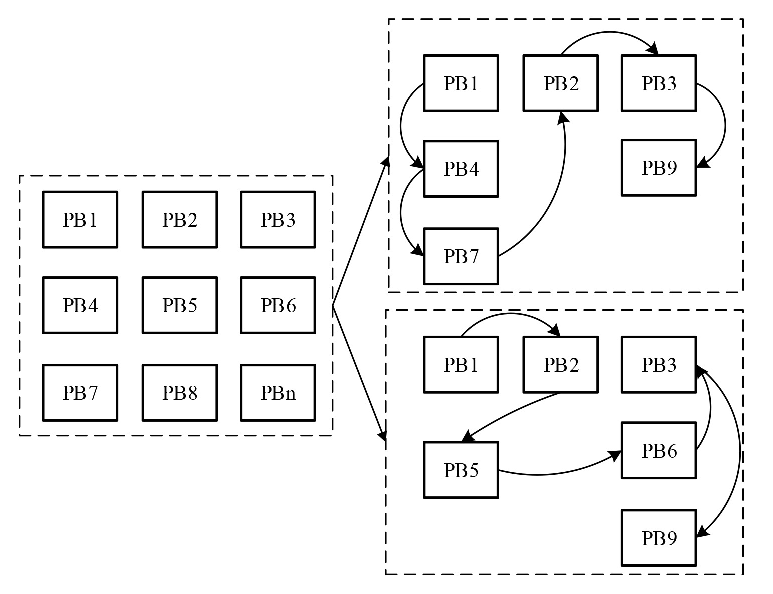
\includegraphics[width=3in]{fig/FIG3_TII-18-0024.eps}
\caption{ Customizable control program structure of the $ePLC$,  whose program blocks are independent of each other, and the execution flow is not determined at design time.}
\label{fig:customeprogram}
\end{figure}

With the purpose of separating function development and process development, we used a three-layer development architecture, as shown in Fig. \ref{fig:threelayerarchitecture}:
\begin{enumerate}
\item Engine Layer. In the Engine Layer, the kernel and algorithms are developed through C language or an assembler language by professional developers. The program developed in this layer is called the Engine Program ($EP$), which includes the initialization, interruption handling, timer, communication, and all kinds of algorithms of the $ePLC$. The motion control-related algorithms are also included in the engine program.

\item Control Program Layer. In the Control Program Layer, programs can be written by the languages in IEC61131-3. Engineers with no knowledge of programming can program the PLC easily through graphical languages, such as LD, SFC, and FBD. The programs developed in this layer are called Control Program ($CP$), which includes logic control and motion control. The motion control-related function is realized by calling the algorithms in the $EP$, and the execution sequence and parameters are of no concern in this layer's program.


\item Application Customizing Layer. In the application customizing layer, users can customize the sequence and parameters of motion control. The customizing program is concerned with the special control process, and it is implemented through calling the program modules in the $CP$ layer. Users can program in this layer, and the $ePLC$ can compile it into the $CP$ layer in real time. The program developed in this layer is called the Application Customizing Program ($ACP$).


\end{enumerate}

\begin{figure}
\centering
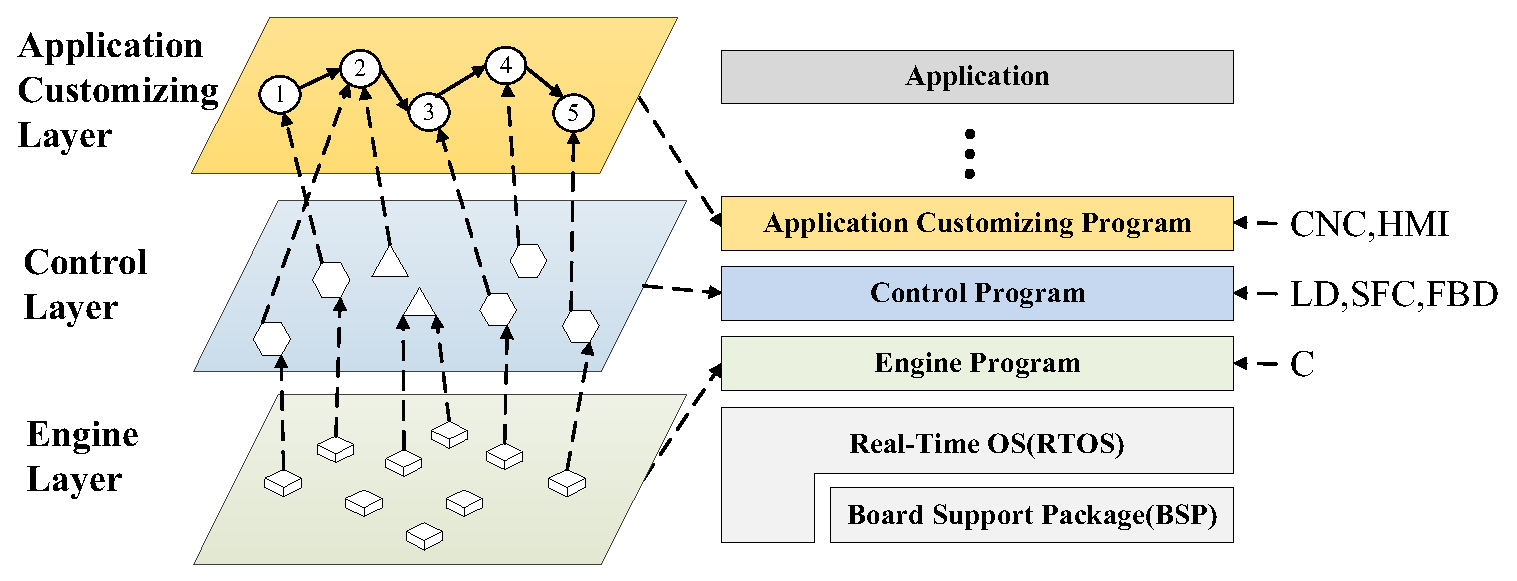
\includegraphics[width=3.5in]{fig/FIG4_TII-18-0024.eps}
\caption{Three-layer architecture of the ePLC.}
\label{fig:threelayerarchitecture}
\end{figure}


A complex control system can be divided into three comparatively simple parts through the aforementioned architecture, and the flexibility is also improved tremendously. Developers are independent of each other so that they can focus on their own task; meanwhile, the motion control part in the $CP$ is application-independent through the introduction of the $ACP$ layer, which can make the $CP$ stable. An application developer can customize and adjust the motion $CP$ via the $ACP$ according to  actual requirements. Compared with the way that the $ACP$ directly calls algorithms in the engine layer, the $CP$ layer can not only implement the task of logic control, but also make the adjustment of motion control more easily. Programs of each layer are stored in fixed positions of PLC's FLASH, and the programs will be moved to RAM when the power is on. The following discussions are in the case that programs are running in RAM.

\subsection{Thread Relationship Analysis}
The $ePLC$ used a priority-based preemptive multi-thread scheduling system, with four priorities and six threads, as shown in Fig. \ref{fig:multithreadstructure}. The threads at the same priority level use the time slice to get the run time.


\begin{figure}
\centering
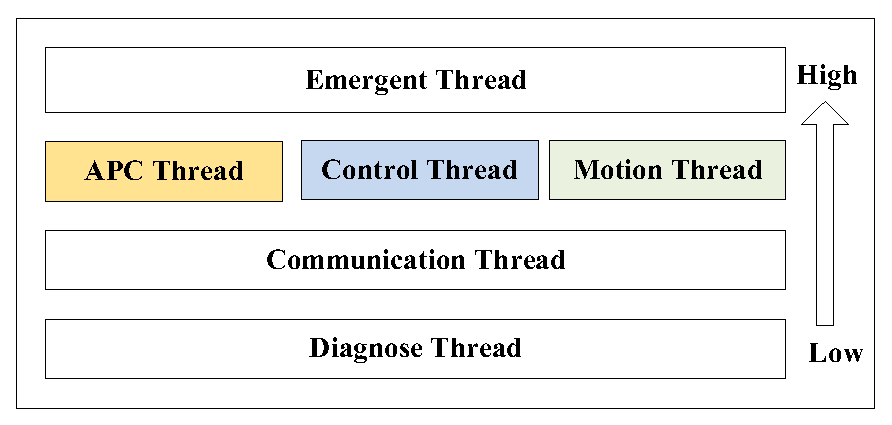
\includegraphics[width=3.5in]{fig/FIG5_TII-18-0024.eps}
\caption{Sketch map of multi-thread structure, including four priorities and six threads.}
\label{fig:multithreadstructure}
\end{figure}



\textbf{Emergent Thread}: The emergent thread has the highest priority and is used to handle emergent tasks, such as interrupts. All interrupts, including I/O interrupts, timer interrupts, exception interrupts, and so on, unless they are caused by fatal errors, will not be handled immediately when occurring. The interrupt information will be packaged and pushed to a queue that will be handled by the emergent thread.


\textbf{ACP Thread}, \textbf{Control Thread}, and \textbf{Motion Thread}: The $ACP$ Thread, Control Thread, and Motion Thread have the same priority. The $ACP$ Thread is used to handle the $ACP$ by reading, parsing, and executing the program. The Control Thread is used to handle the $CP$, responding to the requests of the $ACP$ thread and calling engine algorithms to run. The Motion Thread is used to respond to the requests of the Control Thread and to execute the algorithms in the $EP$ to output the motor-driven signals. The purpose of the corporation of multi-threads is to avoid task blockages caused by task delays in multi-task systems, and thus to improve the system's responsiveness. For example, when the Motion Thread is waiting for the end of the actuator, I/O logical control can work as normal.


\textbf{Communication Thread}: The Communication Thread is used to deal with the communication task, and responds to all kinds of communication requests, such as HMI.

\textbf{Diagnose Thread}: A diagnosis module was embedded in the system, and the idle time of the CPU was used to diagnose nonfatal faults on the condition of not affecting control function.


\subsection{Relation and Definition of Data Interaction}
Communication, synchronization, and mutual exclusion between multi-threads must be handled correctly and efficiently to ensure that the $ePLC$ can work as expected. In our system, data interaction and parameter passing were realized by shared memory. Similar to PLCs, a public and specific data area in memory was dedicated to store the values of soft elements. Data area D is a byte data area, and is used to realize parameters passing; data area M is a bit data area, and is used to realize synchronization and mutual exclusion. Several specific data regions in data area D and data area M were used to realize data exchange and run control, as exemplified in Fig. \ref{fig:publicdataarea}. These data sections are defined as follows:\\

\textbf{Definition 1} $EAPD$ (Engine Algorithm Parameter Data Section): a specific section in data area D used to store the parameters of engine algorithms; the address of every parameter is fixed.\\

\textbf{Definition 2} $EAFD$ (Engine Algorithm Flag Data Section): a specific section in data area M used to store the start flag, stop flag, and state flag of algorithms. Engine algorithms can be called to execute by setting the start flag in the $CP$, and the algorithm's state can be detected by reading the state flag.\\

\textbf{Definition 3} $ACPDD$ ($ACP$ Dedicated Data Section): a specific section in the RAM used to store the \emph{$ACP$} from FLASH.\\

\textbf{Definition 4} $ACPPSD$ ($ACP$ Parameter Swap Data Section): a specific section in data area D used to store the parameters obtained from parsing the $ACP$. Only the parameters that are used by the next executing instruction are stored in $ACPPSD$. The $CP$ gets parameters from $ACPPSD$, and passes them to EAPD.\\

\textbf{Definition 5} $ACPTD$ ($ACP$ Trigger Data Section): a specific section in data area M used to start the program block in the $CP$. Every program block is associated with an $ACP$ instruction.

\begin{figure}
\centering
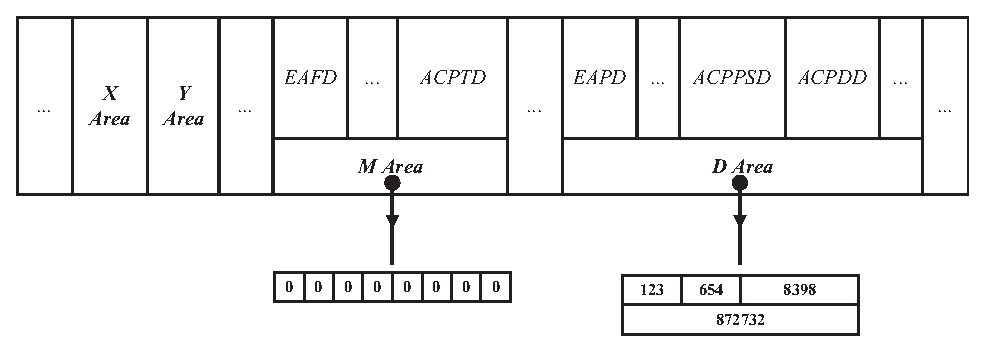
\includegraphics[width=3in]{fig/FIG6_TII-18-0024.eps}
\caption{Distribution of dedicated public data area.}
\label{fig:publicdataarea}
\end{figure}
%%%Fig.6. Distribution of dedicated public data area.
\section{The Realization of Engine and Algorithms}
\label{Engine-Algorithms1}
The $EP$ was responsible for initialization, interrupt handling, timing, communications, and other basic functions ($BF$) of the $ePLC$. It also contained several expansion algorithms ($EA$) that enhanced the $ePLC$'s functionality.Supposing $EP=\{BF,EA,EAP,EAF\}$, $EA=\{ea_1,ea_2,\cdots,ea_i, \cdots , ea_m\}$, which means that the EA contains $m$ algorithms. Corresponding to $m$ algorithms, the $EAP$ is parameter set for $EA$ with $m$ subsets, $EAP=\bigcup_{i=1}^mEAP_i$. $EAP_i=\{eap_1,eap_2,\cdots, eap_i, \cdots , eap_n\}$ is the set of all parameters for $ea_i$, written as
$EAP_i \bowtie ea_i$. Furthermore, $\exists EAP_i \bowtie ea_i \cdot \exists EAP_j \bowtie ea_j : i\neq j \rightarrow EAP_i\cap EAP_j=\emptyset$. $EAF=\bigcup_{i=1}^mEAF_i$ is the flag set for $EA$ with $m$ subsets. $EAF_i= \{eaf_1, eaf_2, \cdots,eaf_i, \cdots, eaf_k\}$ contains $k$ flags used to start and indicate the state of algorithms for $ea_i$, written as $EAF_i\bowtie ea_i$. Additionally, $\exists EAF_i\bowtie ea_i  \cdot \exists EAF_j \bowtie ea_j:i\neq j \rightarrow EAF_i \cap EAF_j=\emptyset$.
The set of trigger flags $TS=\{on,off\}$, is triggered by the upper layer, and cleared by the $EP$. The set of running state $RS = \{run,stop\}$, is set and cleared in the $EP$. The state is set to $run$ after sending running signals to the actuator, and the state is set to $stop$ when the actuator stops working. Therefore, $run$ and $stop$ can also indicate the state of the algorithm. Cartesian product $TS\times RS$ represents all possible combination of the states; in other words, any value of $EAS_i$  belongs to $TS \times RS$.
$<off,stop>$ means the $Stop$ state of the engine algorithm; in this state, when the trigger flag switches from $off$ to $on$, $<on,stop>$ is used to indicate that the algorithm is in the $Ready$ state, and can be scheduled to execute by the thread at any time. The trigger flag was cleared before executing to avoid repeated execution, and the $stop$ was switched to $run$ at the same time to indicate that the algorithm was in a running state; then, the $Stop$ state was transited to $Run$. When the algorithm finished running, the $run$ flag was switched to $stop$ again, and the state transited to $Stop$. Fig.\ref{fig:statetransition} illustrates the state transition.

\begin{figure}
\centering
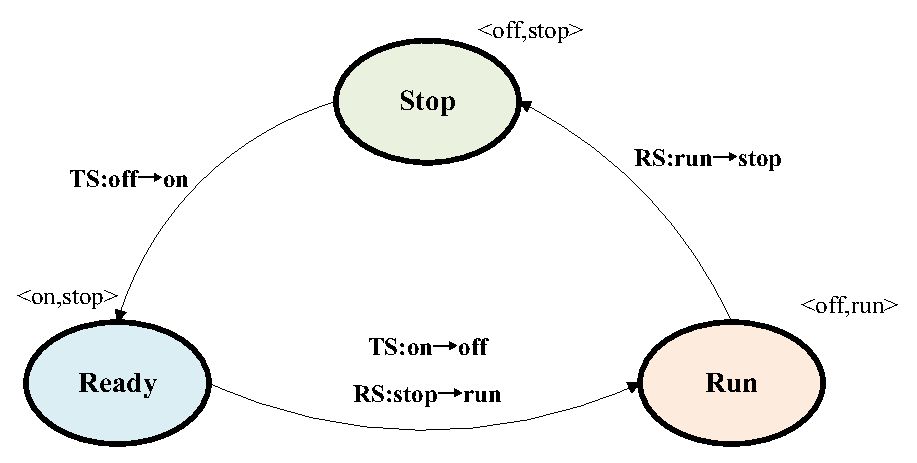
\includegraphics[width=3in]{fig/FIG7_TII-18-0024.eps}
\caption{State transition diagrams of engine algorithms.}
\label{fig:statetransition}
\end{figure}



\section{Design and Realization of the ACP in the ePLC}
\label{ACP-PLC2}
The $ACP$ layer was used to customize motion sequence and parameters. It includes programming, compiling, and executing. An $ACP$ is composed of a list of $ACP$ instructions. An $ACP$ instruction is an atomic unit of the $ACP$, and every instruction implements a single function. Each $ACP$ is made up of several instructions that are executed in chronological order. In our system, every $ACP$ instruction was used to pass parameters and set the program block of $CP$ to run. Therefore, we first needed to design the $ACP$ instruction.
\subsection{Design and Realization of the ACP Instruction}
Supposing the instruction set has $m$ instructions, $IS=\{I_1,I_2,\cdots,I_m\}$, $I_i=(name,code,P)$. Any instruction has a name, a code, and a parameter set $P$. The instruction name is a mnemonic symbol to demonstrate the instruction's function. The instruction code is unique and can be used to identify an instruction, namely $\neg \exists I_i \exists I_j:I_i.code==I_j.code\wedge i\neq j$. We adopted a natural number $N$ as the instruction code in the instruction set.
 In the development environment of the PC, only the instruction name and parameters were used, and the instruction format was defined as shown below:\\
$I_i.name \quad I_i.p_1,I_i.p_2,I_i.p_3,\cdots,I_i.p_n$.\\
Any $ACP$ program consisted of a finite number of chronological instructions.
\subsection{Compilation and Execution of ACP}
\subsubsection{Compilation}
Compiling the $ACP$ means converting the $ACP$ to $ACP\textquoteright$, which can be identified and executed by the $ePLC$, $f:ACP \rightarrow ACP\textquoteright$. It contained two steps, $f=g\circ h$.
% * <karyns@accdon.com> 2017-12-25T07:42:57.410Z:
% 
% > \textquoteright$
% Please correct this throughout this section.
% 
% ^.
Function g transformed the instruction name to an instruction code, $g: ACP \rightarrow T$, $g(I_i.name)=I_i.code,i=0,1,\cdots,m$. Obviously, $g$ is a one-to-one function.
Function $h$ normalized parameters, $h:T\rightarrow ACP\textquoteright$. The objective of $h$ was to transform parameters to a standard format. For readability, we used a non-standardized format, which is easy for users to understand. The non-standardized format is denormalized; for example, the pulses of movement are a normalized expression of distance. In order to make it easy to understand for the user, centimeters were used as the non-standardized format for distance. Thus, parameters were normalized by transforming the parameters to the format accepted by the $ePLC$.

The data frame downloaded into the $ePLC$ was made up of compiled instructions and an END flag, as shown in fig.\ref{fig:formatofACPprogram}. In order to parse the $ACP$ conveniently, the length of each parameter was 4 bytes long. The data frame was parsed by the $ACP$ driver module when the $ePLC$ was running.

\begin{figure}
\centering
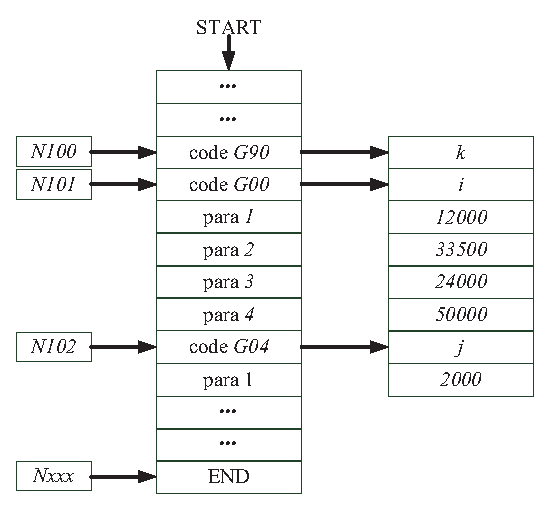
\includegraphics[width=3in]{fig/FIG8_TII-18-0024.eps}
\caption{Format of the $ACP$ frame after compiling.}
\label{fig:formatofACPprogram}
\end{figure}


\subsubsection{Parsing and Executing the ACP}
The $ACP$ driver module read every $ACP$ instruction from the $ACPDD$, and obtained parameters by parsing the instruction. The parameters were passed to $ACPPSD$.
The information necessary for parsing the instruction was saved in a table $PT$, where each row corresponded to an instruction. $PT=\{pi_1,pi_2, \cdots ,pi_m\}$, and the number of table rows was equal to the number of  $ACP$ instructions. $pi_i=(code,np,pea,ta)$, and the $code$ of $pi_i$ was the same as the instruction code mentioned above. np is the number of parameters for instruction $i$. Because we denoted that the length of each parameter was 4 bytes, the length of the data block moved to $ACPPSD$ could be determined by $np$. $pea$ is the address of $ACPPSD$, which is the offset of the starting address of area $D$. $ta$ is the starting address of the trigger flag data section, which is the offset of the starting address of area $M$. Every bit in the trigger flag data section was used to control the execution of a function module in the $CP$, and the instruction code could be used as an offset within the byte.
The parsing and execution process included the following steps:\\
\textbf{Step 1}: Reading instructions. Read a byte from the current pointer position $DP$ of $ACPDD$ as the $ACP$ instruction code, and judge whether it is the end of program. If yes, stop the process; if not, go to step 2.\\
\textbf{Step 2}: Parsing instruction. Get the necessary information for instruction parsing from table $PT$ according to the instruction code.\\
\textbf{Step 3}: Transferring Data. Pass the parameters of the current instruction to $ACPPSD$ according to $np$ and $pea$, which are obtained by parsing the instruction. The 4$\times np$ bytes data in $ACPDD$ following the position of the code are moved to the address of $Dstart+pea$, as illustrated in Fig.\ref{fig:parametersfromACPDDtoACPSD}.\\
\textbf{Step 4}: Execution instruction. Set the corresponding bit of $ACPTD$ to 1 according to ta and the instruction code, as shown in Fig.\ref{fig:settingexecutionbitinACPTD}. The bit data in area $M$ was used as the trigger flag in the $CP$, and $ta$ indicates the offset to the start address of area $M$. The instruction code was taken as the offset within the byte to get the bit needed to be set 1(ON) in order to execute the corresponding program block in the $CP$.\\
\textbf{Step 5}: Waiting for the end of execution. The $ACP$ thread will wait until the end of the execution, and then go to step 1 again.

These steps are carried out repeatedly until all instructions are handled.
\begin{figure}
\centering
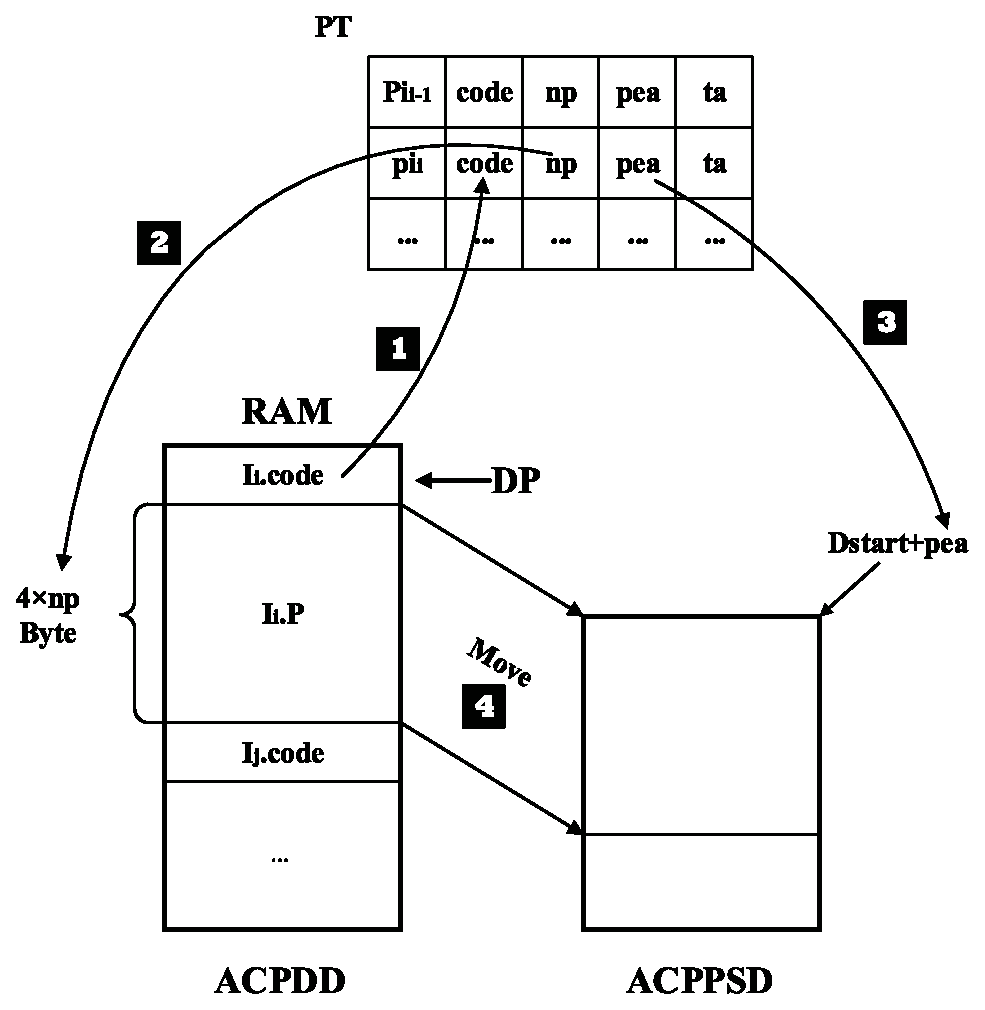
\includegraphics[width=3in]{fig/FIG9_TII-18-0024.eps}
\caption{Schematic of delivering $ACP$ instruction parameters from $ACPDD$ to $ACPPSD$.}
\label{fig:parametersfromACPDDtoACPSD}
\end{figure}



\begin{figure}
\centering
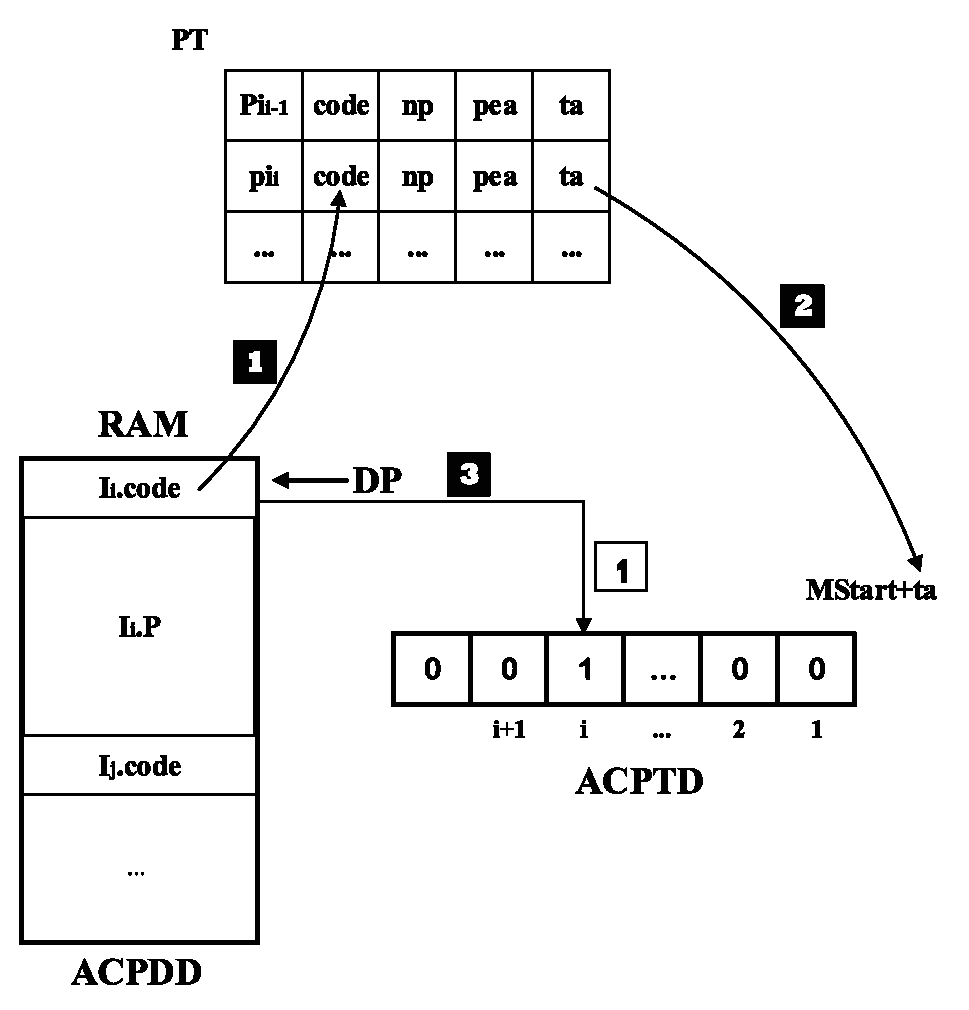
\includegraphics[width=3in]{fig/FIG10_TII-18-0024.eps}
\caption{ Schematic of setting the execution bit in $ACPTD$.}
\label{fig:settingexecutionbitinACPTD}
\end{figure}



\section{Implementation of the PLC Control Program}
\label{PLC-Control-Program3}
The $CP$ was developed using  IEC61131-3 standard languages, which includes LD, SFC, FBD, ST, and IL. LD is a graphic programming language that is widely used to develop control algorithms for PLCs. In this paper, we took LD as the programming language. The $CP$ was the middle level of our three-layer architecture, and it not only responded to the request of the top $ACP$ layer, but also called the algorithms in the engine layer.
$CP=\{IP,LP,MC,MS\}$, where $IP$ is the initial program, which implements the initial operation of data area, port, and state. $LP$ is the logical part of the $CP$.$MC$ is the motion control part of the $CP$. $MC=\{mc_1,mc_2,\cdots,mc_m\}$, where $mc_i$ is used to realize the $i_{th}$ $ACP$ instruction, and the instruction code is $i$. $MS$ is a set of flags used to control $MC$, $MS=\{ms_1,ms_2,\cdots,ms_m\}$, and $ms_i$ is used to trigger the execution of $mc_i$, as shown in fig.\ref{fig:bitdatainM}. Any $ms_i$ contains two states: $ON$ and $OFF$. When the state is switched from $OFF$ to $ON$, the corresponding $mc_i$ will execute. In the $ePLC$, the data $M$ area can be used as a control flag, and thus every program block of $MC$ takes a bit of $M$ to control it.
\begin{figure}
\centering
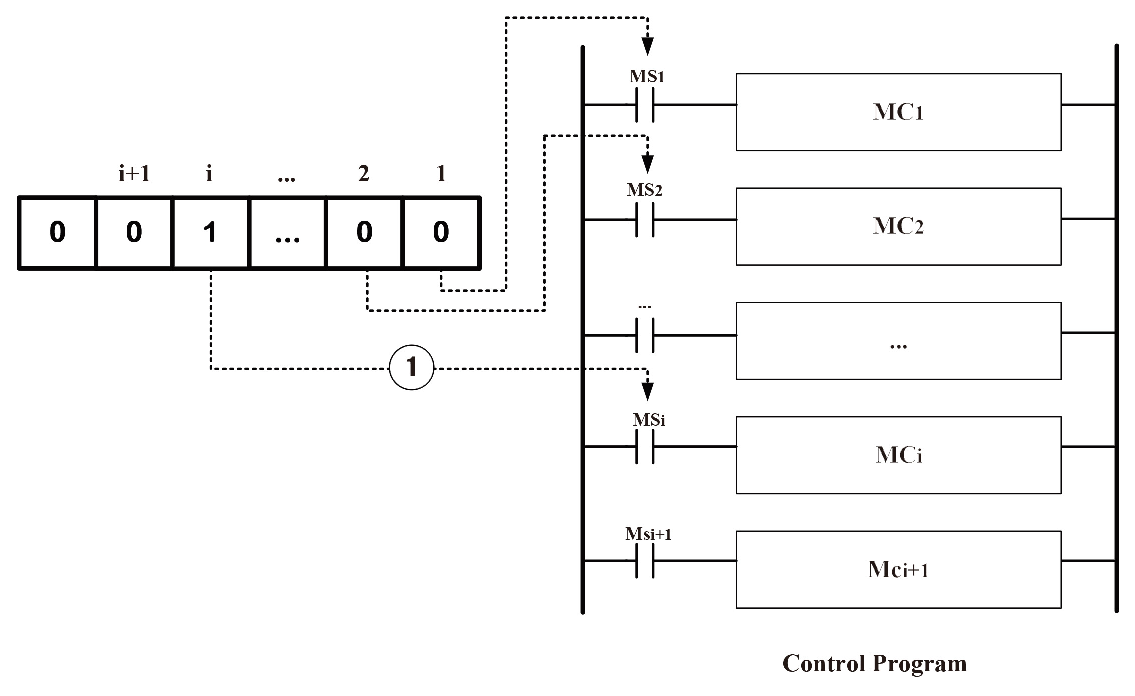
\includegraphics[width=3.5in]{fig/FIG11_TII-18-0024.eps}
\caption{Using bit data in area M to control the program module's execution.}
\label{fig:bitdatainM}
\end{figure}


The $mc_i$ implements the function of passing parameters, condition judgment, and algorithm calling. The parameters were moved to $EAD$, and $T$ of $EAS_j$ was set to $ON$ before $mc_i$ called the subset $EA_j$ of EA.
Besides logical control, the motion control part of the $CP$ was called by thread cyclicly, which included the following steps:\\
\textbf{Step 1}: Traversing $ACPTD$ to judge whether there is any suspended $ACP$ instruction. If yes, go to step 2; otherwise, finish this cycle.\\
\textbf{Step 2}: Moving data in $ACPPSD$ to $EAPD$ in accordance with the agreed format.\\
\textbf{Step 3}: Setting the corresponding bit in $EAFD$ to execute the algorithm in the $EP$ and clear suspended bits in $ACPTD$.\\
\textbf{Step 4}: Reading the running state bit of the algorithms in $EAFD$ on each loop to wait for the end of execution. At the end of execution the loop will go to step 1 to start the next cycle.\\

\section{Collaboration of Threads}
\label{Collaboration-Threads}
The synchronization and mutual exclusion of the $ACP$ thread and the Control Thread were realized by semaphore $T_1$. The synchronization and mutual exclusion of the Control Thread and the algorithm thread were realized by semaphore $T_2$. The $ACP$ thread contained the following five steps.\\
\textbf{Step 1}: Reading instruction ($p_1$).\\
\textbf{Step 2}: Parsing instruction ($p_2$).\\
\textbf{Step 3}: Acquiring execution semaphore $T_1$($p_3$).\\
\textbf{Step 4}: Passing data ($p_4$).\\
\textbf{Step 5}: Starting up execution ($p_5$).\\
The Control Thread includes the following five steps.\\
\textbf{Step 1}: Executing logical $CP$ ($q_1$).\\
\textbf{Step 2}: Traversing the flag section of the $ACP$ instructions, and judging whether there are $ACP$ instructions needed to be executed ($q_2$).\\
\textbf{Step 3}: Acquiring execution semaphore T1, and T2 ($q_3$).\\
\textbf{Step 4}: Passing data of $ACPPSD$ to $EAPD$ ($q_4$).\\
\textbf{Step 5}: Calling the engine algorithm to execute by setting the corresponding control flag, and returning $T_1$($q_5$).\\
The Algorithm Thread contains the following four steps.\\
\textbf{Step 1}: Traversing the flag section of algorithm execution, and judging whether there is any algorithm needed to be executed (s1).\\
\textbf{Step 2}: Acquiring semaphore T2 (s2).\\
\textbf{Step 3}: Executing the algorithm (s3).\\
\textbf{Step 4}: Waiting for the end of execution, and returning semaphore T2 (s4).\\

\begin{figure*}
\raggedright
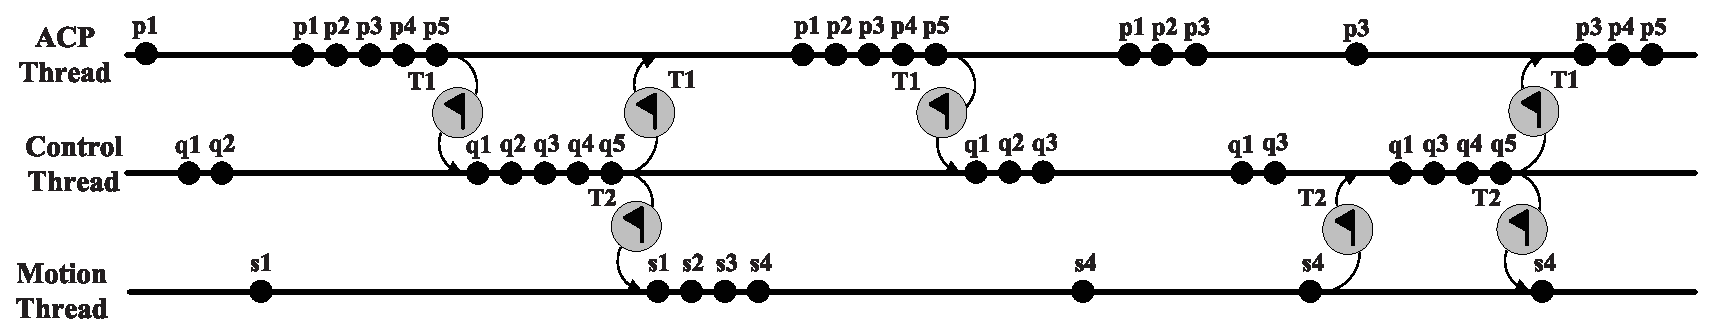
\includegraphics[width=7in,keepaspectratio]{fig/FIG12_TII-18-0024.eps}
\caption{Collaboration of threads.}
\label{fig:The corporation of threads}
\end{figure*}
 
The process was as follows. First, the $ACP$ thread reads instructions ($p_1$)from $ACPDD$. When there is an $ACP$ instruction needed to be executed, the $ACP$ driver module will parse the instruction to get the necessary information to execute the instruction ($p_2$). Then, it attempts to acquire semaphore $T_1$ ($p_3$). Once done, parameters will be moved to $ACPPSD$ ($p_4$), and the corresponding flag bit in $ACPTD$ will be set ON ($p_5$). Then, semaphore $T_1$ is returned to the Control Thread, and the next cycle starts. If the thread cannot get the semaphore $T_1$, it will keep trying until success.
Besides logical control ($q_1$), the Control Thread traverses $ACPTD$ ($q_2$) to judge whether there is an $ACP$ instruction needed to be executed; if yes,it tries to acquire the semaphores $T_1$, $T_2$ ($q_3$). After getting the semaphores $T_1$ and $T_2$, parameters are moved from $ACPPSD$ to $EAPD$ ($q_4$). Then, the corresponding flag bit in $EAFD$ is set to $ON$ in order to execute the algorithm. Then, the semaphores $T_1$ and $T_2$ will be released. When there is a suspended $ACP$ instruction needed to be executed and the thread cannot get the semaphores $T_1$ or $T_2$, the Control Thread continually executes $q_1$ and $q_3$ until it get the semaphores $T_1$ and $T_2$.
The algorithm thread traverses $EAFD$ continuously to judge whether there is an algorithm needed to be executed ($s_1$); if yes, it tries to acquire the semaphore $T_2$ ($s_2$). After getting semaphore $T_2$, the corresponding algorithm will be executed ($s_3$) to generate signals for the actuator, and waits for the actuator to stop running ($s_4$). The semaphore $T_2$ will be released after the end of running.
\begin{figure}
\centering
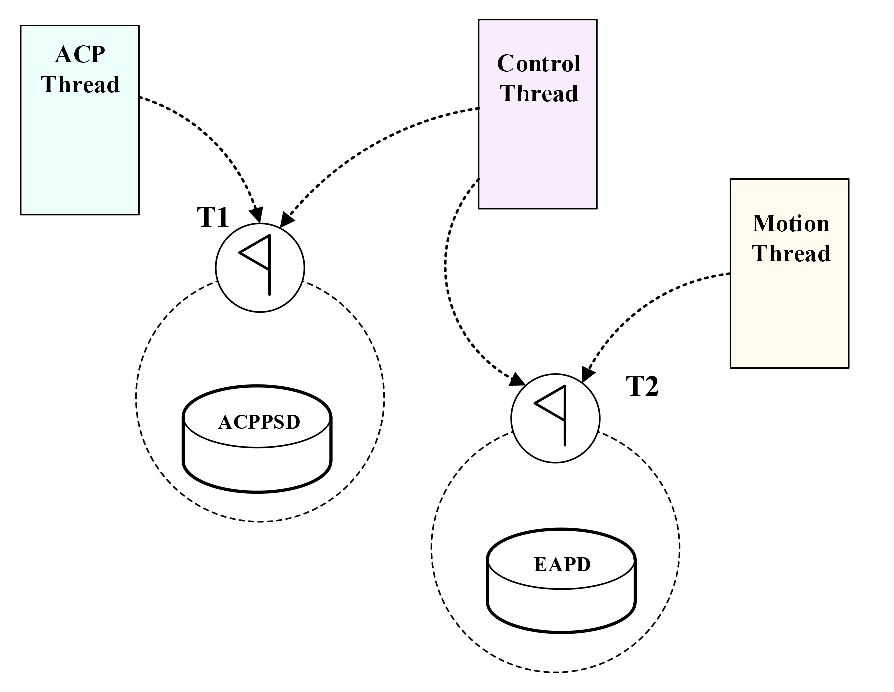
\includegraphics[width=3in]{fig/FIG13_TII-18-0024.eps}
\caption{Mechanism of data sharing and exclusion between threads.}
\label{fig:datasharing}
\end{figure}
Data sharing of threads was realized through shared memory. In order to protect data and ensure their consistency, different threads were not allowed to operate on the same data area simultaneously. Due to the use of a multi-layer structure in our system, only the adjacent layer threads operated on the same data area. As shown in fig.\ref{fig:datasharing}, semaphore $T_1$ was used to realize the mutual exclusion of $ACPPSD$. The $ACP$ thread could write $ACPPSD$ only when it got the semaphore $T_1$; meanwhile, the Control Thread could read $ACPPSD$ only when it got the semaphore $T_1$. Similarly, the Control Thread and the algorithm thread realized the mutual exclusion of $EAPD$ via semaphore $T_2$.

\section{Case Analysis}
\label{Case-Analysis}


\subsection{Introduction of the Experiment Equipment}
An automatic winding machine was used in our experiment, as shown in Fig.\ref{fig:machine}.
\begin{figure}
	\centering
	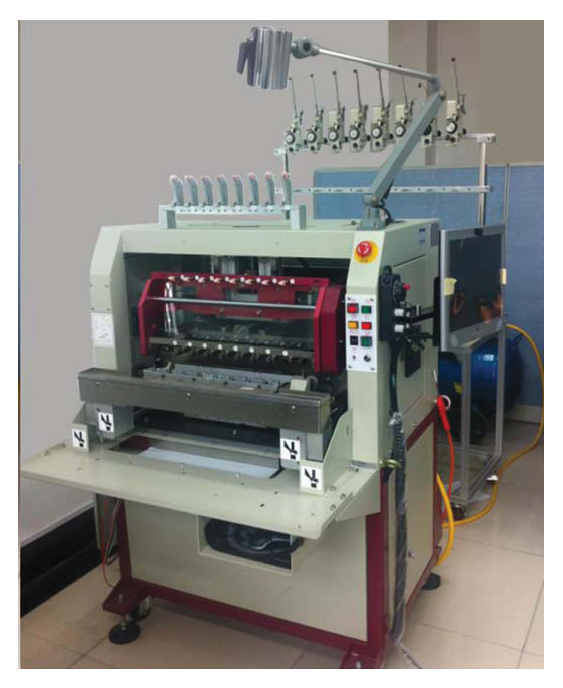
\includegraphics[width=2.5in]{fig/FIG14_TII-18-0024.eps}
	\caption{Automatic winding machine.}
	\label{fig:machine}
\end{figure}
The machine had five cooperating axes and twelve air pumps to implement the function of wire arrangement, winding pins, trimming, loading and unloading the skeleton, and so on. The five axes were the X-axis, Y-axis, Z-axis, U-axis, and Q-axis. The X-axis, Y-axis, and Z-axis were responsible for cable feeding and coiling operation, and the executors were servo motors. As the master axis, the U-axis was responsible for winding, and the executor was also a servo motor. The Q-axis was used to control the winding angle, and the executor was a stepping motor.
The controller of the winding machine was an $ePLC$ CASS-PLCA149B with motion control, which we developed ourselves, as shown in Fig.\ref{fig:controlboard}. The controller used a dual-processor architecture, and was composed of two STM32 CortexM3 chips. The controller had 32 input ports, 32 output ports, and six motor interfaces. The main processor and the slave processor worked cooperatively to control the motor running. The main processor sent parameters and command signals to the slave processor, which generated PWM pulses and other control signals for the motors. The $ACP$ program, $CP$, and motion algorithm in the $EP$ were executed in the main processor.

\begin{figure}
	\centering
	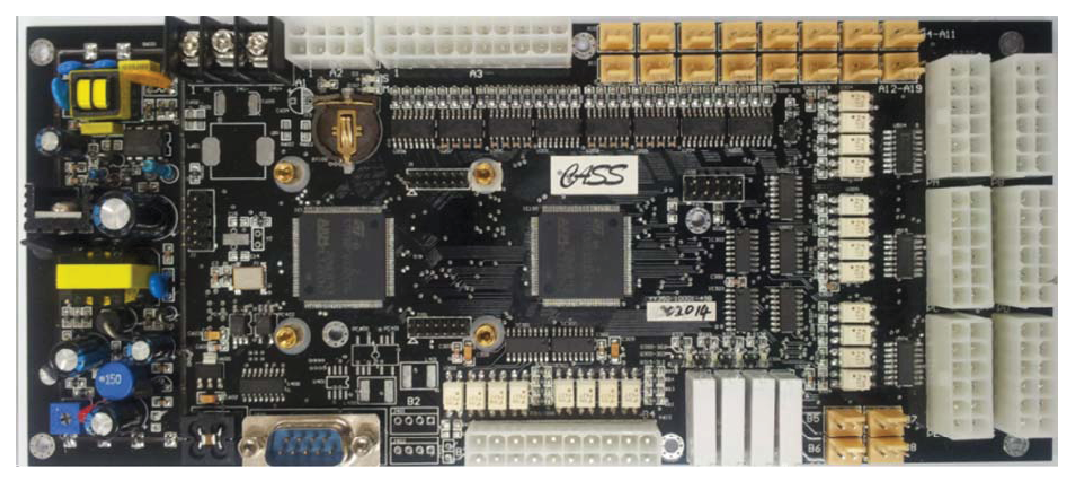
\includegraphics[width=3in]{fig/FIG15_TII-18-0024.eps}
	\caption{Photo of ePLC CASS-PLCA149B.}
	\label{fig:controlboard}
\end{figure}
\subsection{Action Analysis of the Winding Machine}
Only the control of the motors was considered here. The movement driven by the air pumps was not discussed in this paper because they can be realized easily by I/O control in the $CP$. The winding machine could perform the following actions:

\begin{enumerate}
	\item	Reset: First, the X-axis, Y-axis, Z-axis, U-axis, and Q-axis search for the Z point through z-phase positioning. Then, each axis moves a given distance, and at last the location of each axis is set as its origin.
	\item	Loading skeletons: At the beginning of coiling, the combined movement of the air pumps carries the skeletons from the material platform to the U-axis.
	\item	Unloading skeletons: At the end of coiling, the combined movement of the air pumps carries the skeletons from the U-axis to the material platform.
	\item   Linear feed: Motors drive the X-axis, Y-axis, and Z-axis, respectively, to make the guide pin, which is used to guide a copper wire to a specified location.
	\item	Winding pin: This task is implemented by the X-axis, Y-axis, and Z-axis working cooperatively. The X-axis and Y-axis perform circular movements with a specified radius. Meanwhile, the Z-axis ascends or descends according to a specified distance. In this step, the copper wire is fixed on the pin of the skeleton.
	\item	Winding: The U-axis drives the skeleton to rotate in high-speed. The X-axis is the slave-axis, and moves back and forth following the U-axis. The copper wire winds on the skeleton when the X-axis and U-axis perform master–slave movements.
	\item	Trimming: After coiling another pin, the gripper pump moves forward or backward so that the copper wire is pulled apart.

\end{enumerate}


\subsection{ACP Instruction Design and Analysis}
Based on the above analysis we defined the customized winding machine language ($CWML$) as shown in Table \ref{table:result1}. The $CWML$ is a customized streamlined language that included instructions with a customized format. It was primely supported by the proposed software structure on the $ePLC$. In this case, 13 instructions satisfied almost all required applications for winding. Meanwhile, the proposed three-layer structure supported adding instructions easily, and the Application Customizing Layer could compile the $ACP$ in real time. 

It would be hard work to implement our approach with some widely used languages, such as G-Code, which is shown in Table \ref{table:GCODE}. It includes 217 instructions, and every instruction contains several parameters. 
\begin{table}
	\scriptsize \caption{The definition of CWML}
	\label{table:result1}
	\begin{center}
		\renewcommand{\arraystretch}{1.4}
		\setlength\tabcolsep{3pt}
		\begin{tabular}{|p{0.3cm}|p{2cm}|p{0.7cm}|p{2cm}|p{2cm}|}
			\hline
			No. & Code & Params & Description & Function\\
			\hline
			01  & R00 X\_Y\_Z\_S\_ & 4 & X: X-axis distance Y: Y-axis distance Z: Z-axis distance S: Speed & X, Y, Z-axis high-speed feed \\
			\hline
			02  & R00 U\_ S\_ & 2 & U: U-axis distance S: Speed & U-axis high-speed feed \\
			\hline
			03  & R00 Q\_ S\_ & 2 & Q: Q-axis distance S: Speed & Q-axis high-speed feed \\
			\hline
			04  & R00CW X\_N\_D\_FD\_BD\_S\_  & 4 & X: X-axis distance N: Number of turns D: Wire diameter FD: Forward decreasing distance BD: Backward decreasing distance S: Speed & U-axis clockwise winding \\
			\hline
			05  & R00CCW X\_N\_D\_FD\_BD\_S\_ & 4 & X: X-axis distance N: Number of turns D: Wire diameter FD: Forward decreasing distance BD: Backward decreasing distance S: Speed & U-axis counterclockwise winding \\
			\hline
			06  & R02CW R\_N\_Z\_S\_ 	 & 4 & R: Circle radius N: Number of turns Z: Z-axis distance S: Speed & Clockwise winding pin \\
			\hline
			07  & R02CCW R\_N\_Z\_S\_ & 4 & R: Circle radius N: Number of turns Z: Z-axis distance S: Speed & Counterclockwise winding pin \\
			\hline
			08  & R04 & 1 & T: delay time & Pause \\
			\hline
			09  & R05	 & 0 &  & Absolute coordinate \\
			\hline
			10  & R06	 & 0 &  & Incremental coordinate \\
			\hline
			11  & R07 & 1 &  & Gripper output \\
			\hline
			12 & R08 & 1 &  & Load skeleton\\
			\hline
			13 & R09 & 1 &  & Discarding waste wire\\
			\hline
		\end{tabular}
	\end{center}
\end{table}


\begin{table}
	\scriptsize \caption{List of G-Code found on FANUC}
	\label{table:GCODE}
	\begin{center}
		\renewcommand{\arraystretch}{1.4}
		\setlength\tabcolsep{3pt}
		\begin{tabular}{|p{0.3cm}|p{2cm}|p{0.7cm}|p{4cm}|}
			\hline
			No. & Code & Params & Description\\
			\hline
			01  & G00 X\_Y\_Z  & 3 & Rapid positioning \\
			\hline
			02  & G01 X\_Y\_Z & 3 & Linear interpolation\\
			\hline
			03  & G02 X\_Y\_R\_F & 4 & 	Circular interpolation, clockwise \\
			\hline
			...  & ...  & ... & ... \\
			\hline
			101  & G100  & 0 & Tool length measurement \\
			\hline
			102  & M00 & 0 & Compulsory stop \\
			\hline
			103  & M01 & 0 & Optional stop \\
			\hline
			104  & M03 & 0 & Spindle on (clockwise rotation) \\
			\hline
			...  & ... & ... & ... \\
			\hline
			201  & M99 & 0 & Subprogram end \\
			\hline
			202  & N01 & 0 & Turn on load monitor \\
			\hline
			203  & N02 & 0 & Inch units. Absolute mode. Activate work offset. Activate tool offset. Deactivate tool nose radius compensation. \\
			\hline
			... & ... & ... & ...\\
			\hline
			217 & N16 & 0 & Program stop, rewind to top of program, wait for cycle start\\
			\hline
		\end{tabular}
	\end{center}
\end{table}

We could develop, debug, and compile the $ACP$ in ComEditorX, which is as an Integrated Development Environment(IDE) for $ACP$. ComEditorX could be used to both develop the $ACP$ program and supply a means to define customized $ACP$ instructions.


\subsection{Experimental Result}
The $EP$ was divided into master and slave parts, which were executed in the master and slave processors separately. The master $EP$ contained the motion control algorithm, $CP$ driver module, and $ACP$ program driver module, in addition to basic functions. The slave program was used to generate signals for the motors according to commands from the master.


The $CP$ was developed in a graphical IDE for the $ePLC$ using the LD language. In the IDE we could program, debug, and compile\cite{A40} the $CP$.
The $CP$ was downloaded to the $ePLC$ after compiling.


Once the $EP$ and $CP$ were developed and downloaded to the $ePLC$, users could develop the $ACP$ for the winding machine. Under a given skeleton and wire diameter, users could optimize the motion control sequence and parameters of the $ACP$ repeatedly in the single step mode. Finally, the $ACP$ was downloaded to the $ePLC$. 

The skeleton was winded as in Fig.\ref{fig:result}. In this case, the diameter was 0.6 $mm$, the distance was 20 $mm$, the velocity was 40 $mm/s$, and the number of turns was 4. Table \ref{table:ComparisonG} compares the winding programs of G-Code and CWML. Because G-Code is designed for CNC, its velocity is low in most cases, the unit of instruction of G01 and M03 are $mm/min$ and $RPM$, respectively. We found that the $CWML$ was much easier to use than G-Code in the winding machine.

Fig.\ref{fig:result_2}  shows the other products of the winding machine. If the skeleton, wire diameter, or position of the pin were changed, only the parameters of the $ACP$ required adjustment. The $CP$ and $EP$ did not need to change. 

\begin{table}
	\scriptsize \caption{Comparison between G-Code and CWML}
	\label{table:ComparisonG}
	\begin{center}
		\renewcommand{\arraystretch}{1.4}
		\setlength\tabcolsep{3pt}
		\begin{tabular}{|p{0.3cm}|p{2.5cm}|p{4.2cm}|}
			\hline
			No. & G-Code & CWML\\
			\hline
			01  & M03 S400 & R00CW X20 N4 D0.6 FD0.3 BD0.3 S40\\
			\hline
			02  & G01 X20 F2400 &\\
			\hline
			03  & G01 X0.3 F2400 &\\
			\hline
			04  & G01 X19.7 F2400 &\\
			\hline
			05  & G01 X0.6 F2400 &\\
			\hline
			06  & G01 X19.4 F2400 &\\
			\hline
			07  & G01 X0.9 F2400 &\\
			\hline
			08  & G01 X19.1 F2400 &\\
			\hline
			09  & G01 X0 F2400 &\\
			\hline
			10  & M05 &\\
			\hline
		\end{tabular}
	\end{center}
\end{table}



\begin{figure}
	\centering
	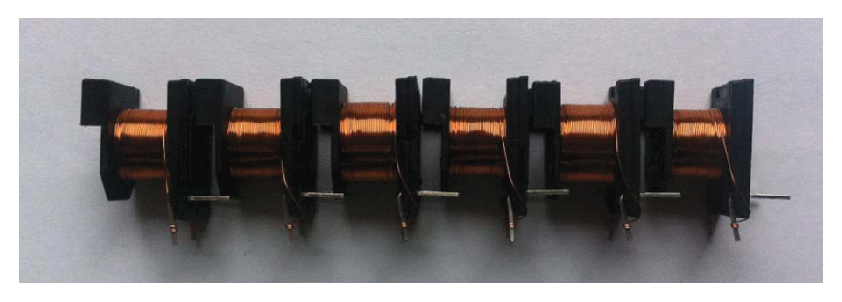
\includegraphics[width=3in]{fig/FIG16_TII-18-0024.eps}
	\caption{Product of the winding machine.}
	\label{fig:result}
\end{figure}

\begin{figure}
	\centering
	
\includegraphics[width=3in]{fig/FIG17_TII-18-0024.eps}
	\caption{Other winding skeletons.}
	\label{fig:result_2}
\end{figure}


  
\section{Conclusion}
\label{conclusion}
In this paper we proposed a customized real-time compilation method to simplify special motion control. The concept of an $ePLC$ and a three-layer development architecture were put forward. The description method and compiled algorithm of the architecture were introduced in detail. Based on the software structure on the $ePLC$, we proposed the $CWML$, which was then applied to a winding machine. Using this development method, we can expand the applications of the $ePLC$ to robotics, numerical control machines, and so on.



\ifCLASSOPTIONcaptionsoff
  \newpage
\fi



% trigger a \newpage just before the given reference
% number - used to balance the columns on the last page
% adjust value as needed - may need to be readjusted if
% the document is modified later
%\IEEEtriggeratref{8}
% The "triggered" command can be changed if desired:
%\IEEEtriggercmd{\enlargethispage{-5in}}

% references section

% can use a bibliography generated by BibTeX as a .bbl file
% BibTeX documentation can be easily obtained at:
% http://www.ctan.org/tex-archive/biblio/bibtex/contrib/doc/
% The IEEEtran BibTeX style support page is at:
% http://www.michaelshell.org/tex/ieeetran/bibtex/
%\bibliographystyle{IEEEtran}
% argument is your BibTeX string definitions and bibliography database(s)
%\bibliography{IEEEabrv,../bib/paper}
%
% <OR> manually copy in the resultant .bbl file
% set second argument of \begin to the number of references
% (used to reserve space for the reference number labels box)

\bibliographystyle{IEEEtran}
\bibliography{reference}

% biography section
%
% If you have an EPS/PDF photo (graphicx package needed) extra braces are
% needed around the contents of the optional argument to biography to prevent
% the LaTeX parser from getting confused when it sees the complicated
% \includegraphics command within an optional argument. (You could create
% your own custom macro containing the \includegraphics command to make things
% simpler here.)
%\begin{IEEEbiography}[{\includegraphics[width=1in,height=1.25in,clip,keepaspectratio]{mshell}}]{Michael Shell}
% or if you just want to reserve a space for a photo:

\begin{IEEEbiography}[{\includegraphics[width=1in,height=1.25in,clip,keepaspectratio]{fig/Author_HuifengWu.eps}}]{Huifeng Wu} received the Ph.D. degree in computer science and technology from Zhejiang university, Hangzhou, China, in 2006. He is currently a professor in the institute of intelligent and software Technology, Hangzhou Dianzi University. His research interests include software development methods and tools, software architecture, embedded system, intelligent control \& automation.
	
\end{IEEEbiography}
\begin{IEEEbiography}[{\includegraphics[width=1in,height=1.25in,clip,keepaspectratio]{fig/Author_YiYan.eps}}]{Yi Yan} received B.S. in automatic control engineering form Zhejiang Sci-Tech University in 1984, M.S. in computer engineering from Beijing University of Postal Telecommunications in 1990. Currently he is the director and full professor in institute of intelligent and software Technology, Hangzhou Dianzi University. His research interests include embedded system, advanced manufacturing system, intelligent control \& automation, and intelligent instruments.
	
	
\end{IEEEbiography}
\begin{IEEEbiography}[{\includegraphics[width=1in,height=1.25in,clip,keepaspectratio]{fig/Author_DanfengSun.eps}}]{Danfeng Sun} received M.S. in computer architecture from Hangzhou DianZi University in 2011. He is currently a research assistant in the Institute of Industrial Internet, Hangzhou DianZi University. His research interests include embeded system, motion control and IIoT.
\end{IEEEbiography}
\begin{IEEEbiography}[{\includegraphics[width=1in,height=1.25in,keepaspectratio,angle=-90]{fig/Author_ReneSimon.eps}}]{Rene Simon} obtained a doctor of engineering at the Otto-von-Guericke University Magdeburg in 2001. He is Professor of Control Systems at the Department of Automation and Computer Sciences, Harz University of Applied Sciences, Wernigerode, Germany. His major research fields include engineering of automation systems, especially industrial controllers. He is chairman of PLCopen and project leader IEC 61131-10 Ed. 1.0.
\end{IEEEbiography}



% insert where needed to balance the two columns on the last page with
% biographies
%\newpage


% You can push biographies down or up by placing
% a \vfill before or after them. The appropriate
% use of \vfill depends on what kind of text is
% on the last page and whether or not the columns
% are being equalized.

%\vfill

% Can be used to pull up biographies so that the bottom of the last one
% is flush with the other column.
%\enlargethispage{-5in}



% that's all folks
\end{document}


